\chapter{Examining Partial Circuits}

% FIXME - somewhere I need to be sure I state the requirements for doing power calculations with AC (i.e., RMS provides the average power that it will use in any direction)

We will end our discussion of amplification by discussing partial circuits.
Often times you will need to design a circuit which connects to another circuit, either powering it or receiving power from it.
For instance, in the amplification circuits from Chapter~\ref{chapTransVoltageAmp}, the outputs were connected to a speaker.
They could also be connected to another amplifier, or to a stomp box (a device to modulate the incoming signal in some way), or a recording circuit.

\section{The Need for a Model}

In order to connect circuits together, we need to be able to describe, in general terms, the ways that circuits fit together.
In our early attempts to analyze circuits, we looked at how we could combine a lot of resistors in series and parallel to come up with a single resistance for the whole circuit.

When dealing with transistors and other power amplification devices, we often need to come up with a simplified model for how the input to a circuit or the output from a circuit behaves.
Early on (in Chapter~\ref{chSeriesParallel}), we learned how to take multiple resistors in series and parallel and combine them into an equivalent single resistor.

When dealing with a power amplification circuit, it is often necessary look at various parts of the circuit by themselves, and figure out how they \emph{look} to other parts of the circuit.
The way that a partial circuit looks to other parts of the circuit is called the circuit's \glossterm{\thev Equivalent} circuit.

\simplepdffigure{A Complicated Circuit and its \thev Equivalent Circuit}{TheveninEquivalentExample}{0.25}

A \thev equivalent circuit takes a partial circuit and reduces it to:

\begin{itemize}
\item A single voltage source (AC, DC, or DC-biased AC, expressed in RMS voltage)
\item A single impedance (i.e., resistance) in series with the voltage source
\end{itemize}

Note that the single voltage source may be \emph{different} than the voltage source that is actually connected.
What you are doing is see what the circuit looks like to another circuit.
For instance, a voltage divider circuit makes the output of the voltage divider \emph{look like} it is coming from a lower voltage source.

Figure~\ref{figTheveninEquivalentExample} shows a circuit and its \thev Equivalent circuit.
For purposes of thinking about and understanding the relationship between the circuit and things attached to the circuit, we can view the circuit as being the same as its \thev Equivalent.
Thus, having a \thev Equivalent circuit greatly simplifies our modeling, calculating, and understanding of how circuits work together.

Any network of power sources and resistances can be converted into a \thev Equivalent circuit.
You can also get a \thev Equivalent circuit for a circuit that includes capacitors and inductors, but the calculations become more difficult and the results are only valid for a specific frequency (each frequency will have a different \thev Equivalent circuit).
For simplicity we will just focus on resistive circuits.

\section{Calculating \thev  Equivalent Values}

% FIXME - somewhere I need to note that resistors hanging off the end don't count for Thevenin voltage

\simplepdffigure{A Voltage Divider Partial Circuit}{TheveninDividerBasic}{0.25}

To see how to calculate the voltage and resistance for a \thev Equivalent circuit, this section will take a classic voltage divider circuit and analyze how it ``looks'' to other attached circuits.
Figure~\ref{figTheveninDividerBasic} shows an example of a partial circuit.
Like most partial circuits, this circuit has two output points---A and B.
What we are wanting to know is this---if we attach another circuit up to A and B, is there a model that we can use to understand how the other circuit ``sees'' our circuit?
The goal of a making a \thev Equivalent circuit is to understand what our circuit will look like to other attached circuits.

So, since our \thev Equivalent circuit will have a voltage source and a single resistor, we need to calculate what the voltage and resistance of this circuit will be.
To calculate the voltage, find out what the voltage of the circuit at the output is when there is \emph{nothing connected}.
That is, if we were to leave A and B disconnected, and I were to connect my multimeter to A and B, what would the voltage be?
This is your \thev voltage.
Since this is a voltage divider, you can just use normal voltage divider calculations to find this out.
In this case, we have a $12\myvolt$ source, and the voltage divider divides it exactly in half ($1\mykohm$ for each half).
Therefore, the output voltage is $6\myvolt$.  
Therefore, our \thev Equivalent circuit will have a $6\myvolt$ source.

Now we need to find our \thev resistance.
There are multiple tricks to do this, but the simplest one is to replace all voltage sources in your circuit with a wire (i.e., a short circuit), and simply compute the total resistance between A and B.\footnote{We haven't talked about \emph{current} sources much in this book.  However, for completeness, I should note that if you have a current source, you should replace it with an open circuit (i.e., a gap in the wire) when calculating \thev resistance.}

\simplepdffigure{Calculating the \thev Resistance of the Circuit}{TheveninDividerBasicForResistance}{0.25}

Figure~\ref{figTheveninDividerBasicForResistance} shows what this looks like.
Therefore, to calculate the \thev resistance of this circuit, simply calculate the total resistance from A to B.
In this case, there are two parallel paths from A to B---one through the first resistor and one through the second.
Therefore, we add up the resistors as parallel resistances.
As a result, our \thev resistance will be:

\begin{align*}
R_T &= \frac{1}{\frac{1}{R_1} + \frac{1}{R_2}} \\
    &= \frac{1}{\frac{1}{1000} + \frac{1}{1000}} \\
    &= \frac{1}{0.001 + 0.001} \\
    &= \frac{1}{0.002} \\
    &= 500\myohm
\end{align*}

Therefore, we would say that this partial circuit has a \thev voltage of $6\myvolt$ and a \thev resistance of $500\myohm$.
Whenever we attach a circuit to this circuit, what that other circuit will ``see'' is a circuit like the one in Figure~\ref{figTheveninEquivalentBasic}.

\simplepdffigure{The \thev Equivalent of the Voltage Divider}{TheveninEquivalentBasic}{0.25}

If you wanted to prove this to yourself, you can imagine a variety of different circuits attached to both our original circuit and to the \thev Equivalent circuit.
You will find that, in all cases, the amount of voltage and current the \thev Equivalent circuit provides to the other circuit is the exact same as what the original circuit will provide.

That isn't to say that the circuits themselves are exactly equivalent.
Our original voltage divider uses up a lot of current stepping down the voltage of the voltage source.
Not only does that waste energy from our battery, but it probably also causes a lot of heat.
However, \emph{the subcircuit that gets attached to A and B} will see both our original circuit and the \thev Equivalent circuit as providing the same output.

\section{Another Way of Calculating \thev Resistance}

There is another way of calculating \thev resistance.  
In this method, we first calculate what the current would be if you shorted A to B directly with a wire.
This is known as the short-circuit current, or $I_{SHORT}$.
Then, after calculating this, you can divide the \thev voltage by $I_{SHORT}$ to obtain the \thev resistance.

When doing this, you have to remember that anything in parallel with our short will be essentially ignored---the current will always want to go through our short circuit.

\simplepdffigure{Finding the Short Circuit Voltage}{TheveninDividerABShort}{0.25}

Figure~\ref{figTheveninDividerABShort} shows what this looks like.
What we want to do is to calculate the current going from A to B.
Since A to B is a short circuit in parallel with our second resistor, we know that \emph{all} of the current will prefer the short circuit.
This means that the current going through A and B will simply be the current that is limited by the first resistor.

So, since we have a $12\myvolt$ source and a $1\mykohm$ resistor, the short circuit current will be:

\begin{align*}
I_{SHORT} &= \frac{V}{R} \\
          &= \frac{12}{1000} \\
          &= 0.012\myamp
\end{align*}

Now, to determine the \thev resistance, we divide the \thev voltage by this number:

\begin{align*}
R_{Thevenin} &= \frac{V_{Thevenin}}{I_{SHORT}} \\
  &= \frac{6}{0.012} \\
  &= 500\myohm
\end{align*}

As you can see, this is the same value that we got from the previous method.

\section{Finding the \thev Equivalent of an AC Circuit with Reactive Elements}

If a circuit has reactive elements (inductors and capacitors), we have to do a little more work to find the \thev Equivalent circuit.

For DC circuits, this is relatively simple. 
Since capacitors block DC currents and inductors are a short circuit for DC currents, we can simply treat the capacitors as open circuits (i.e., unconnected) and treat the inductors as short circuits (simple wires).
For AC circuits, you can get a feel for what this will be by assuming the opposite---that capacitors will be short circuits and inductors will be open circuits.

However, if you were to try to solve it explicitly, the problem is a little more difficult.
The problem is that a full analysis of such circuits requires math involving complex numbers (i.e., numbers involving the imaginary unit $i$).  
While the technique is roughly equivalent to adding resistances in series and parallel as we have done before, it is much more difficult to do the math with complex numbers.
For those who want to see this technique in action, I have included more discussion on this topic in Appendix~\ref{appThevEquivAC}.

For the purposes of this book, the previous statements about DC and AC should suffice for a general understanding of how your circuit works.
In this book will typically use this for analyzing circuits that are mixed between AC and DC signals---small AC signals with a DC offset.
We will generally concern ourselves with the DC offset for purposes of computation.

\section{Using \thev Equivalent Descriptions}

Many circuits are described to users of that circuit using \thev Equivalent descriptions.
For instance, many circuits are described by their input or output impedance.
This gives you a rough guide to imagine what will happen if you connect your own circuit to such circuits.
Imagine that you have a circuit that has a \thev Equivalent output impedance of $500\myohms$.
If you connect an output circuit that only has $250\myohm$ of resistance, what do you think that will do to the signal?
Well, since the output of the circuit is equivalent to going through a $500\myohm$ resistor (that's what \thev Equivalence means), then if I connect a $250\myohm$ resistor, then I will have created a voltage divider in which two thirds of the voltage will be dropped by the circuit I am connecting to, and I will only get one third of the output voltage.
On the other hand, if my output circuit is $50,000\myohm$, then the voltage drop within the output circuit is negligible compared to the voltage drop within my circuit.
This means that my circuit will essentially receive the full \thev Equivalent voltage.

We can also use this to calculate the amount of current that our circuit will draw.
Let's say that a circuit yields a \thev Equivalent output of $4\myvolt$ with an $800\myohm$ impedance.
If I connect a $3,000\myohm$ output circuit, how much current will flow?
The total resistance will be $3,800\myohm$, so the current will be $V / R = 4 / 3800 \approx 1.05\mymamp$.

The same is true for connecting an input circuit that you make to an output circuit someone else made.
For instance, speakers and headphones are normally rated as an impedance---$8\myohm$, $16\myohm$, etc.
They aren't, strictly speaking, resistors, but at normal audio frequencies they behave essentially like one---they have a \thev Equivalent impedance (their \thev Equivalent voltage is zero).

\begin{exampleprob}
If I have an output circuit which is \thev Equivalent to $3\myvolt$ RMS and $200\myohm$, and I connect it to a set of $16\myohm$ headphones, what will the power of the headphones be in watts?

We can understand this circuit as simply being a voltage source followed by two resistors in series.
The voltage source will be $3\myvolt$ and the resistances will be $200\myohm$ and $16\myohm$, totalling $216\myohm$.  
The current will therefor be $V / R = 3 / 216 \approx 0.0139 \myamp$.
The voltage drop in the headphones will be $I \cdot R = 0.0139\cdot 16 \approx 0.222\myvolt$.
Therefore the power delivered to the headphones will be $V\cdot I = 0.222 \cdot 0.0139 \approx 0.00309\mywatt$, or $3.09\mymwatt$.
\end{exampleprob}


\section{Finding \thev Equivalent Circuits Experimentally}

In addition to using circuit schematics to determine \thev Equivalent Circuits, it is also possible to determine them experimentally.
This way, if you are unsure of the input or output characteristics of your device, you can measure it yourself.
The problem with measuring it yourself is that it requires attaching a load to the circuit.
Some circuits will fry if a wrongly-sized load is attached.
You have been warned.

The easiest way to determine \thev Equivalency experimentally is rather unsafe, but it will help us understand better why the method works.
Imagine a voltage divider where the bottom resistor has an extremely large resistance---say $100\myMohm$.
In such a voltage divider, the bottom resistor will have almost the entirety of the voltage drop, right?
In fact, if the bottom resistor was infinite, it would in fact have all of the voltage drop.

Because of this, we can determine the \thev Equivalent voltage by measuring the output voltage when there is nothing connected, because no connection means that there is infinite resistance between the output and ground.
Measuring this value will give us the \thev Equivalent voltage.

To determine the \thev Equivalent current, we can short-circuit the output.
When doing this, the \emph{only} impedances to the current will be within the device itself.
Therefore, using Ohm's law, the amount of current this draws will tell us how large of a resistance the output is yielding.

\begin{exampleprob}
If I measure the open-circuit (i.e., disconnected) voltage of the output of an unknown circuit as $8\myvolt$ and the short-circuit current of the output as $10\mymamp$, what is the \thev Equivalent circuit?

To find this out, we simply use Ohm's law.
What resistance would cause an $8\myvolt$ source have $10\mymamp$ of current?

\begin{align*}
R &= V / I \\
  &= 8 / 0.010 \\
  &= 800
\end{align*}

Therefore, our \thev Equivalent circuit is $8\myvolt$ with an impedance of $800\myohm$.
\end{exampleprob}

The problem with this method is that you don't normally want to short circuit your output.  
Additionally, some circuits require some sort of a load to work properly.
In order to adjust to such scenarios, there is a set of equations that allow us to measure the voltage drop across a large and small resistance (instead of infinite and no resistance) and come up with a \thev Equivalent circuit.

The equations are a little complex, but you can actually derive them directly from Ohm's law if you work at it.
The first one calculates the \thev Equivalent voltage ($V_T$) from the voltage with a high resistance ($V_H$), the high resistance value ($R_H$), the voltage with a low resistance ($V_L$), and the low resistance value ($R_L$):

\begin{equation}
\label{eqThevEqVoltExp}
V_T = \frac{\frac{V_H}{R_H}(R_H - R_L)}{1 - \frac{V_H R_L}{R_H V_L}}
\end{equation}

Then, we can calculate the \thev Equivalent resistance:

\begin{equation}
\label{eqThevEqResExp}
R_T = \frac{V_T R_L}{V_L} - R_L
\end{equation}

For a basic starting point, you can use $1\myMohm$ for the high resistance value, and $1\mykohm$ for the low resistance value.

\begin{exampleprob}
I have a circuit that generates an output for which I need to know its \thev Equivalent properties.
I tested the circuit with a $200\myohm$ resistance and a $1000\myohm$ resistance.
With the $200\myohm$ resistance, there was a $2\myvolt$ drop across the resistance.
With the $1000\myohm$ resistance, there was a $5\myvolt$ drop across the resistance.
What is the \thev Equivalent circuit for this circuit?

First we find the \thev Equivalent voltage using Equation~\ref{eqThevEqVoltExp}:

\begin{align*}
V_T &= \frac{\frac{V_H}{R_H}(R_H - R_L)}{1 - \frac{V_H R_L}{R_H V_L}} \\
    &= \frac{\frac{5}{1000}(1000 - 200)}{1 - \frac{5\cdot 200}{1000\cdot 2}} \\
    &= \frac{0.005\cdot800}{1 - \frac{1000}{2000}} \\
    &= \frac{4}{0.5} \\
    &= 8\myvolt
\end{align*}

Next we can find the \thev Equivalent resistance using Equation~\ref{eqThevEqResExp}:

\begin{align*}
R_T &= \frac{V_T R_L}{V_L} - R_L \\
    &= \frac{8\cdot 200}{2} - 200 \\
    &= 800 - 200 \\
    &= 600\myohm
\end{align*}

Therefore, our unknown circuit has a \thev Equivalent voltage of $8\myvolt$ and a \thev Equivalent impedance of $600\myohm$.
\end{exampleprob}

What makes this method valuable is that it allows a way to \emph{experimentally} determine the \thev Equivalent of a partial circuit that you don't have a schematic for, or for which determining the \thev Equivalent circuit might be difficult due to non-linear components such as transistors.

\reviewsection

In this chapter, we learned:

\begin{enumerate}
\item In order to be able to connect circuits together without knowing all of the details of how they are implemented, we need a simplified model of how those circuits work with other circuits they are connected to.
\item A \thev Equivalent circuit is a combination of a single voltage source and a single series impedance which models the way that the given circuit will respond to other attached circuits.
\item To calculate \thev Equivalent voltage, calculate the voltage drop for an open circuit between the two terminals.  This is the \thev Equivalent voltage.
\item To calculate \thev Equivalent impedance, calculate the impedance from one terminal to another (or to ground if there is only one terminal), replacing any voltage sources with short circuits.
\item Alternatively, to calculate \thev Equivalent impedance, calculate the current flowing from one terminal to another if there was a short circuit between them.  Then use Ohm's law to calculate the resistance.
\item \thev Equivalent circuits can be used to understand how the resistances of attached circuits will affect the signal coming out of or into a  circuit.
\item \thev Equivalent circuits can also be found experimentally.  
\item \thev Equivalent voltage can be determined by simply measuring the voltage drop of an open circuit across the terminals.
\item \thev Equivalent resistance can be determined by measuring the current flow of a short circuit across the terminals, though it isn't recommended.
\item Alternatively, given two different load resistances across the terminals, a \thev Equivalent circuit can be calculated using Equations~\ref{eqThevEqVoltExp} and~\ref{eqThevEqResExp}.
\end{enumerate}

\applysection

\begin{enumerate}
\item Why would we want to know what a circuit's \thev Equivalent circuit is?
\item What are the two components of a \thev Equivalent circuit?
\item Think about the two-stage amplifier that you built in Chapter~\ref{chapTransVoltageAmp}.  How would you go about finding the \thev Equivalent circuit as it is seen by the headphones?
\item Suppose I have a circuit where the output terminals have a $2\myvolt$ drop when it is an open circuit, and have $2\mymamp$ of current flowing through it when it is a short circuit.  Draw the \thev Equivalent circuit.
\item If I have a \thev Equivalent circuit of $4\myvolt$ with an impedance of $400\myohm$, what will be the voltage drop of the load if I attach a $2000\myohm$ resistor across the output?
\item If I have a \thev Equivalent circuit of $3\myvolt$ with an impedance of $100\myohm$, what will be the voltage drop, the current, and the power of the load if I attach headphones rated at $32\myohm$?
\item Calculate and draw the \thev Equivalent circuit of the circuit below: 
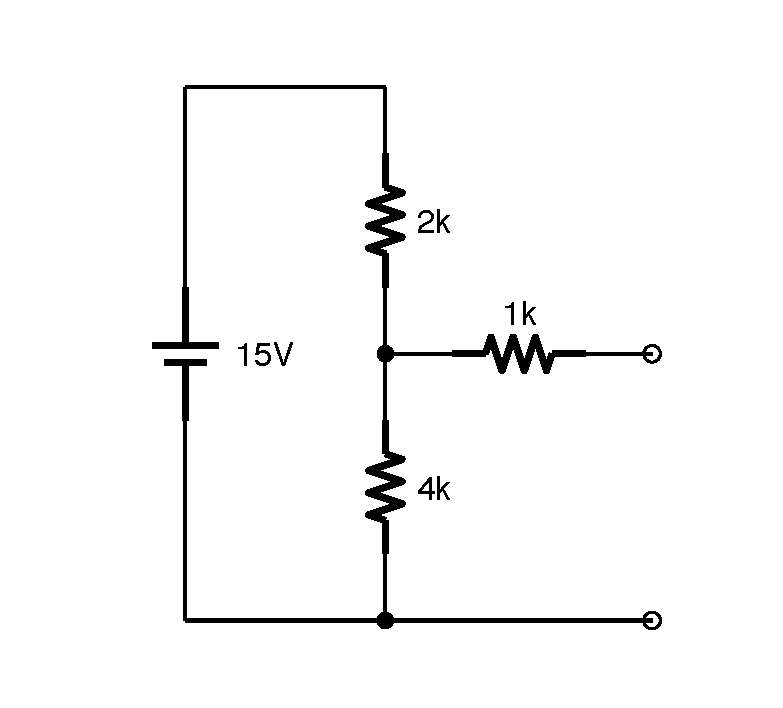
\includegraphics[scale=0.25]{ThevProblem1.pdf}
\item Suppose I have a circuit where, when I add a load of $350\myohm$ I get a $7\myvolt$ drop, and when I add a load of $2000\myohm$ I get an $8\myvolt$ drop.  Calculate and draw the \thev Equivalent circuit.
\end{enumerate}
